%============================================================================
%      PLANTILLA LABORATORIO DE INSTRUMENTACÍON ELECTRÓNICA 
%               INGENIERÍA ELECTRONICA - UNSAAC
%============================================================================

\documentclass[a4paper,12pt]{book}

\renewcommand{\rmdefault}{phv}  % Cambiar la fuente a Helvetica (similar a Arial)
\renewcommand{\sfdefault}{phv}  % Cambiar la fuente sans-serif a Helvetica

\usepackage{./estilos/estiloBase}
\usepackage{./estilos/colores}  
\usepackage{./estilos/comandos} 
\usepackage{graphicx}
\usepackage{subcaption}


\addbibresource{bib.bib}


%\input{Anexo-Siglas.tex}


%%%% PARA LA NOMENCLATURA
\renewcommand{\nomgroup}[1]{%
\ifthenelse{\equal{#1}{A}}{\item[\textbf{T\'erminos Comunes}]}{%
\ifthenelse{\equal{#1}{B}}{\item[\textbf{Caso: URLLC y eMBB}]}{%\\     SE CAMBIA "ESCENARIO" POR "CASO"
\ifthenelse{\equal{#1}{C}}{\item[\textbf{Caso: URLLC y mMTC}]}{%
\ifthenelse{\equal{#1}{D}}{\item[\textbf{Escenario 3}]}{}}}}
}


\begin{document}



\setlength{\parskip}{4mm}	% Separaci??n de los p??rrafos
\overfullrule=2cm			% Muestra una l??nea negra en el borde de la
							% p??gina cuando se superen los m??rgentes
\sloppy						% permite espacios m??s grandes de lo normal
							% para cuadrar las l??neas

%====================== CITAS ============================
\hypersetup{				%Requerido para configurar el comportamiento de los enlaces en el documento
     colorlinks=true,		%Color enlaces (es decir, no más cuadros alrededor de los enlaces)
     linkcolor=blue,		%los enlaces a los archivos locales se establecen en color xxxxxx
     filecolor= yellow,	
     citecolor = blue,  	%color de enlace de citas
     linkbordercolor=white,
     urlcolor=blue,
     pdfborderstyle={/S/U/W 1}}
%====================== CITAS ============================

%\pagestyle{empty}
\begin{titlepage}

  \begin{center}
    \Large{\textbf{UNIVERSIDAD NACIONAL SAN ANTONIO ABAD DEL CUSCO}} \\ 
    \vspace{0.4cm}
    \large{FACULTAD DE INGENIER\'IA EL\'ECTRICA, ELECTR\'ONICA, INFORM\'ATICA Y MEC\'ANICA}\ \\ 
%    \vspace{0.1cm} 
%    \Large{DEPARTAMENTO ACAD\'EMICO DE INGENIER\'IA ELECTR\'ONICA}\ \\ 
    \vspace{0.1cm} 
    \large{ESCUELA PROFESIONAL DE INGENIER\'IA ELECTR\'ONICA}\ \\ 
	
    \vspace{1.0cm}    
    
%    
\includegraphics[width=0.2\textwidth]{images/UNSAAC.png}\\% \hspace{0.1mm} 
    
\includegraphics[width=0.4\textwidth]{images/LI-UNSAAC.png} \\


    \vspace{0.8cm}

    \large{\textbf{\textsc{LABORATORIO DE INSTRUMENTACIÓN ELECTR\'ONICA}}} \\
    \vspace{0.2cm}
    \large{\textbf{\textsc{INFORME PREVIO N° X:}}} \\ 
    
    
    \vspace{0.5cm}
    \large{ \textsc{<<CORRIENTE DE ENTRADA Y DESVÍO EN LA CORRIENTE DE ENTRADA DE AMPLIFICADORES OPERACIONALES>>}} \\
    \vspace{1.0cm}
    
    \begin{table}[H]
    	\centering
    	\begin{tabular}{rl}
    		\large{\textbf{Autor:}}   & \large{Davis Bremdow Salazar Roa}  \\
    		\large{\textbf{Codigo:}}   & \large{200353}  \\
    		\large{\textbf{Docente:}} & \large{Ing. Jose Luis Flores Vasquez}
    	\end{tabular}
    \end{table}

	
	\vspace{0.2cm}

    \Large{Cusco -- Per\'u \\
%    \vspace{0.2cm}
    Septiembre, 2025}
    
  \end{center}
\end{titlepage}

%\cleardoublepage

%\chapter*{Agradecimientos}
%\input{0.1-Agradecimientos}
%\cleardoublepage

%\frontmatter % Introducci??n, ??ndices ...
%\pagestyle{plain}
%\input{0.2-Abstract.tex}
%\cleardoublepage

%\tableofcontents
%\cleardoublepage
%\phantomsection

%\addcontentsline{toc}{chapter}{Resumen}
%\addcontentsline{toc}{chapter}{Abstract}
%\addcontentsline{toc}{chapter}{Resum}

%\listoftables
%\listoffigures

%\mainmatter % Contenido en si ...

%\chapter{Introducci\'on}\label{cap:Introduccion}
\section*{Introducción}

En las diferentes aplicaciones que requieren bajos niveles de tensión o de corriente para el transporte de información el ruido como elemento aditivo ubicado en todo el espectro electromagnético es un parámetros de vital importancia a considerar en este tipo de aplicaciones (biomedica) debido a que su influencia considerable en la medición y/o salida de un sistema, es por tanto que bajo la necesidad de eliminar o trata de reducir de forma significativa tal interferencia que la importancia del amplificador diferencial se utilice como etapa de entrada y el estudio del CMRR un parámetro que permite conocer que tan bien un amplificador diferencial reduce el ruido se tome en consideración antes de elegir un dispositivo en concreto.

En la presente experiencia se abordara la experimentación del amplificador operacional LM741 y la obtención del CMRR (Relación de rechazo en modo común) mediante la obtención de su ganancia diferencial y común en diferentes frecuencias, comprobando además su comportamiento para señales de baja y alta periodicidad.

\section{Medición de resistencias}

Para la experiencia fue necesario contar con los valores precisos para cada resistencia a usar entre las terminales del operacional LM741 debido a que la ganancia diferencia y/o común se encuentran en dependencia de la magnitud de cada una de ellas alterando así la amplificación y/o atenuación en la señal de entrada.

En la tabla \ref{tab:mediciones-resistencias} se muestra las mediciones obtenidas para las resistencias $R_1$, $R_2$, $R_3$ y $R_4$ mostradas en los circuitos \ref{fig:circuito-mod-diferencial} y \ref{fig:circuito-mod-comun} para los modos diferencial y común respectivamente.

\begin{table}[h]
	\centering
	\begin{tabular}{|llll|}
		\hline
		\multicolumn{4}{|c|}{\textbf{Resistencias}}                                                                                                           \\ \hline
		\multicolumn{1}{|l|}{\textbf{R1 {[}K $\Omega${]}}} & \multicolumn{1}{l|}{\textbf{R2 {[}K $\Omega${]}}} & \multicolumn{1}{l|}{\textbf{R3 {[}K $\Omega${]}}} & \textbf{R4 {[}K $\Omega${]}} \\ \hline
		\multicolumn{1}{|l|}{0.989}               & \multicolumn{1}{l|}{9.88}                & \multicolumn{1}{l|}{0.995}               & 9.90                \\ \hline
	\end{tabular}
	\caption{Magnitud Resistencias}
	\label{tab:mediciones-resistencias}
\end{table}

\begin{figure}[h]
	\centering
	\begin{subfigure}[b]{0.45\linewidth}
		\centering
		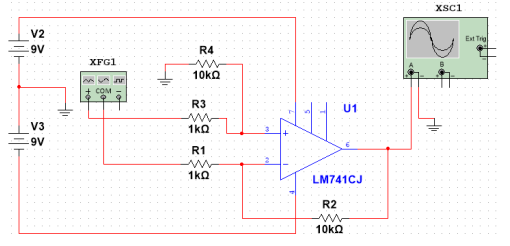
\includegraphics[width=\linewidth]{media/circuito-mod-diferencial}
		\caption{Circuito Amplificador Diferencial - Modo Diferencial}
		\label{fig:circuito-mod-diferencial}	
	\end{subfigure}
	\hfill
	\begin{subfigure}[b]{0.45\linewidth}
		\centering
		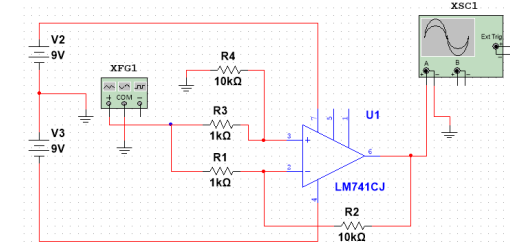
\includegraphics[width=\linewidth]{media/circuito-mod-comun}
		\caption{Amplificador Diferencial - Modo Común}
		\label{fig:circuito-mod-comun}
	\end{subfigure}	
\end{figure}

\section{Ganancia en modo diferencial}

En la figura \ref{fig:imp-circuito-mod-diferencial} se muestra la implementación del circuito del circuito en modo diferencial (referencial) esto debido a que la entrada de retorno se encuentra conectada a tierra, sin embargo para la experimentación este terminal se conecto a la entrada no-inversora del LM741.

\begin{figure}[h]
	\centering
	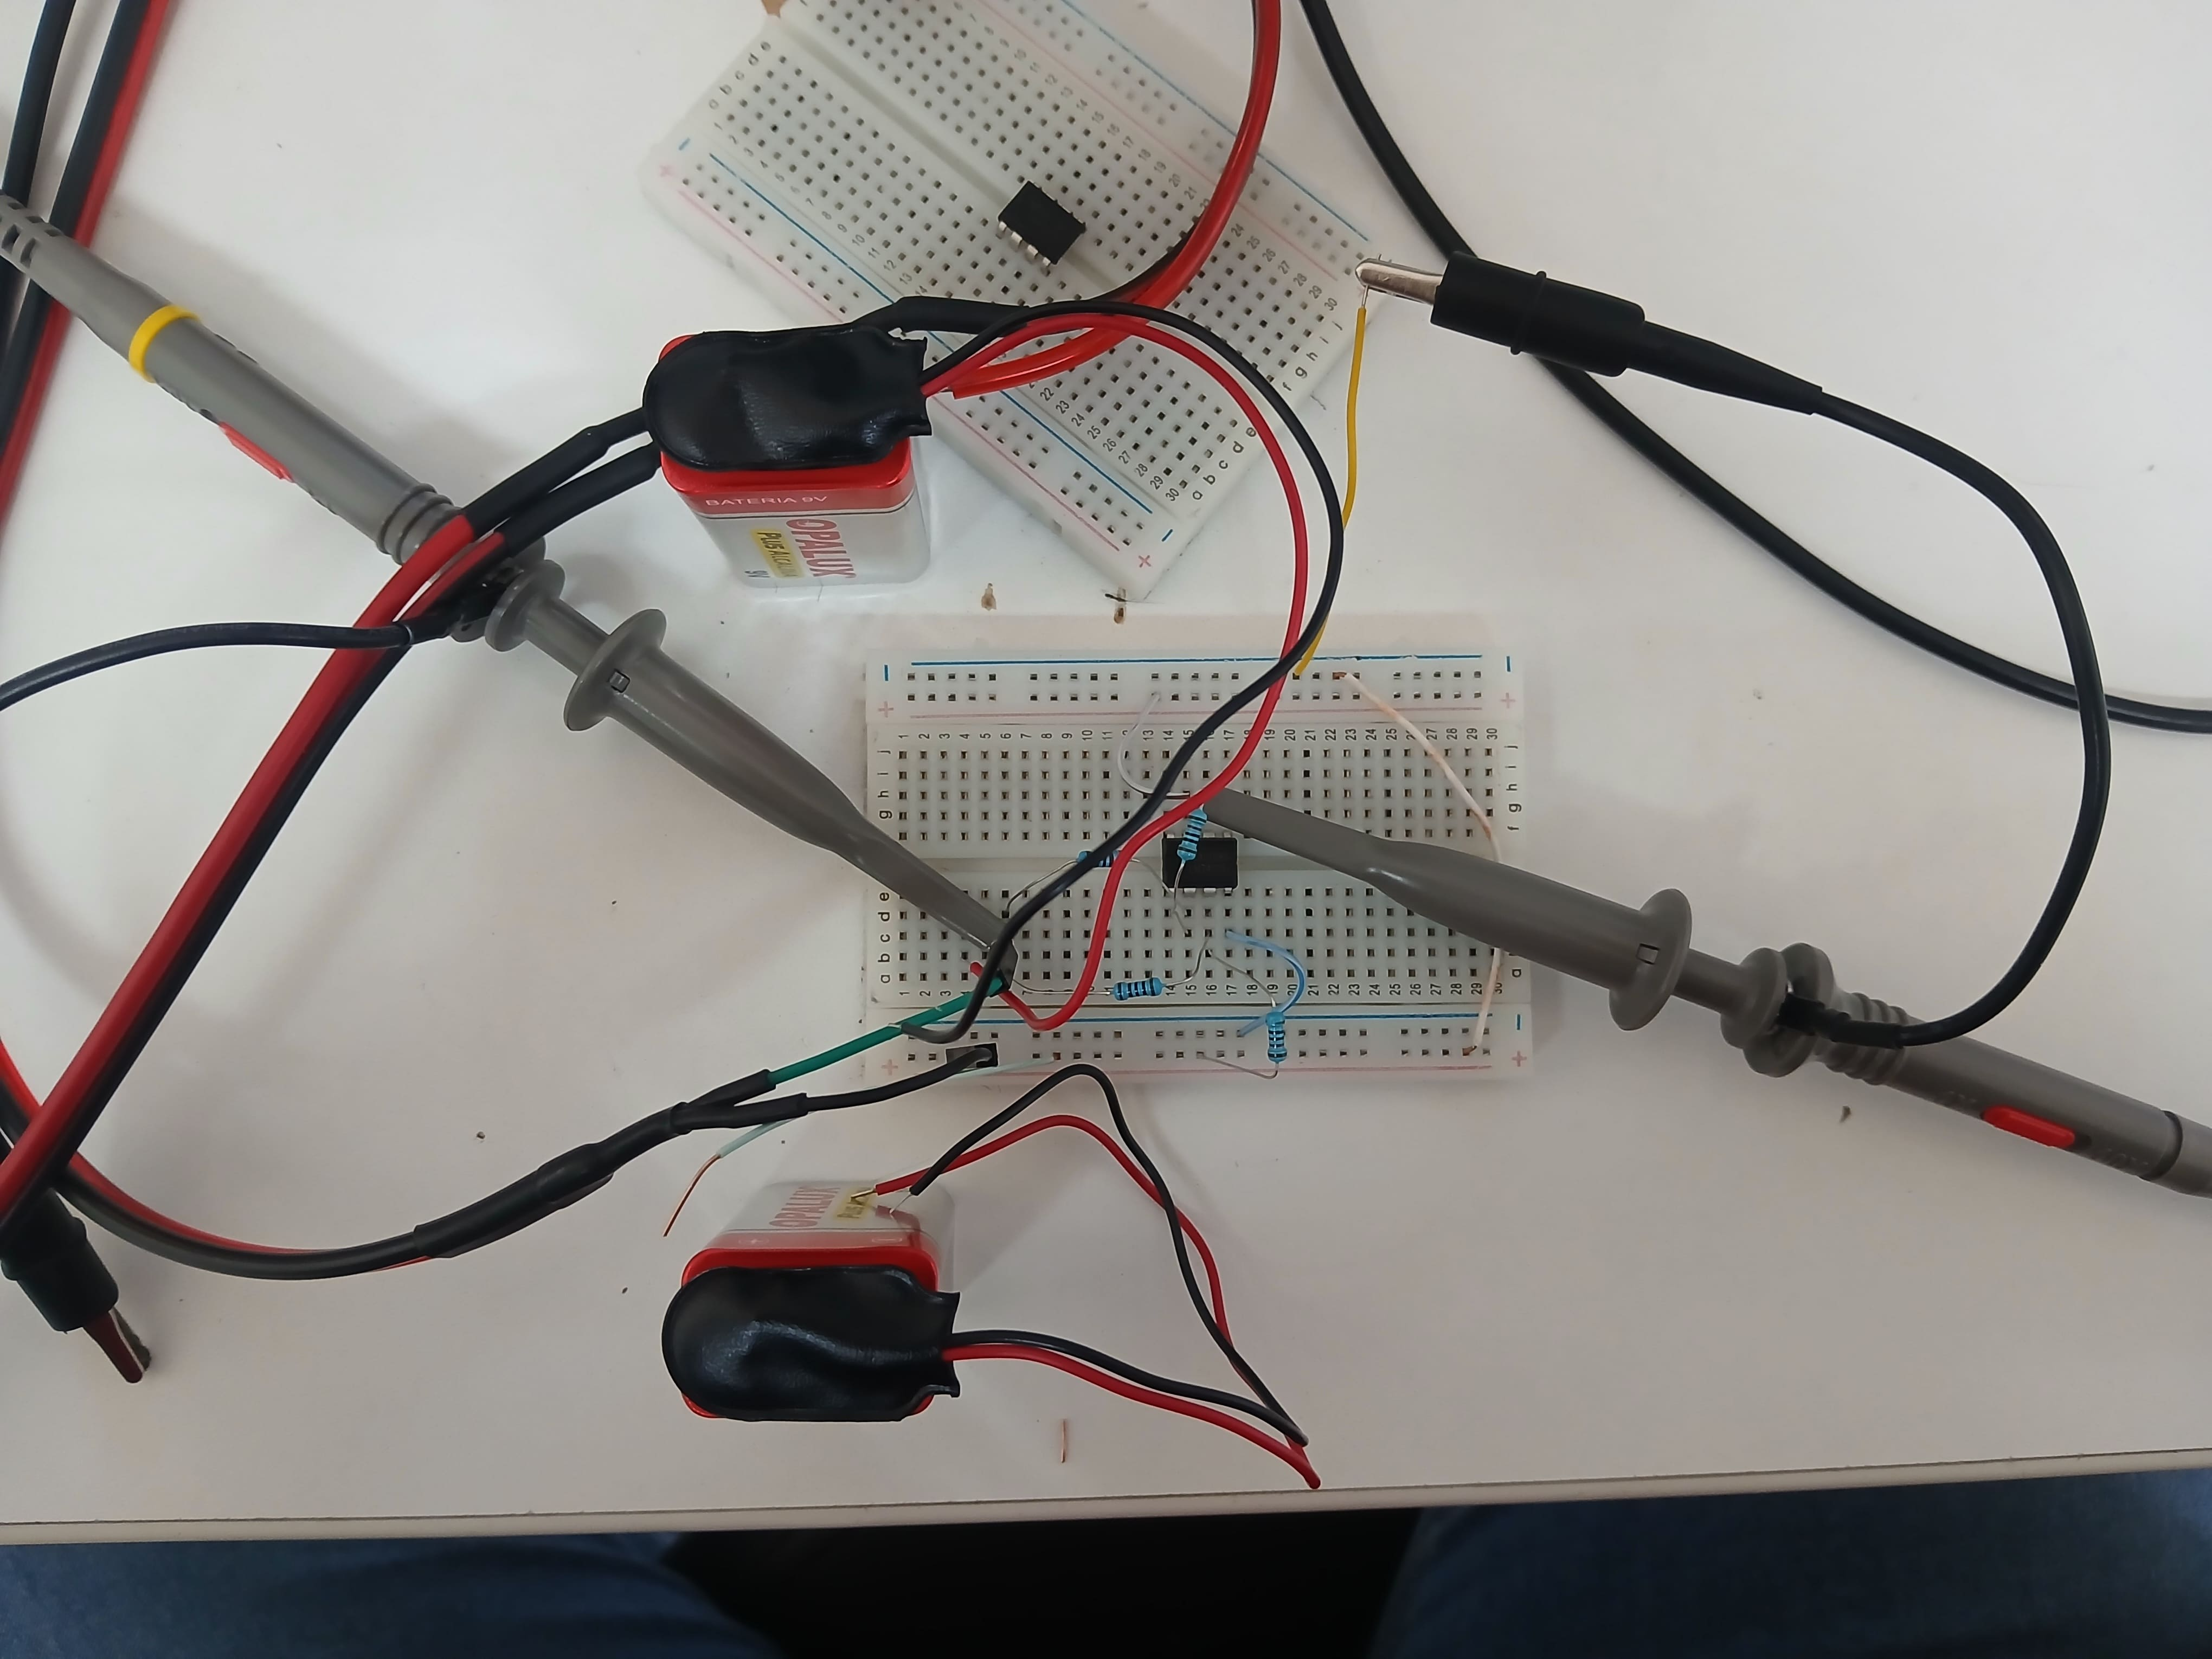
\includegraphics[width=0.5\linewidth]{media/imp-circuito-mod-diferencial}
	\caption{Implementación amplificador diferencial - Modo diferencial}
	\label{fig:imp-circuito-mod-diferencial}
\end{figure}

Por otro lado para proceder con la parte experimental el generador de funciones se configuro para obtener una señal de $500mV_p$ y para un rango de frecuencias entre $500mHz$ hasta los $500KHz$ permitiendo así realizar un análisis de la respuesta en frecuencia del amplificador operacional LM741, esta configuración inicial se puede apreciar en la figura \ref{fig:senial-500mhz-inicial} y con la cual se inicio la experiencia y toma de datos.

\begin{figure}[h]
	\begin{subfigure}[b]{0.45\linewidth}
		\centering
		\includegraphics[width=\linewidth]{"media/MODO COMUN/senial-500mhz-inicial"}
		\caption{Señal sinusoidal de Amp: 500mv y Freq: 500mHz}
		\label{fig:senial-500mhz-inicial}
	\end{subfigure}
	\hfill
	\begin{subfigure}[b]{0.45\linewidth}
		\centering
		\includegraphics[width=\linewidth]{"media/MODO DIFERENCIAL/senial-500mhz-out"}
		\caption{Señal de salida amplificada - Freq: 500mHz}
		\label{fig:senial-500mhz-out}
	\end{subfigure}
\end{figure}


Una vez determinada la señal de entrada se realizo una comparación con la señal de obtenida en el terminal de salida del LM741 observándose la misma señal amplificada en una magnitud de $9.28$ o $19.5361dB$ para la frecuencia de $500mHz$ la salida de esta forma de onda se muestra en la figura \ref{fig:senial-500mhz-out}, utilizando los cursores para la obtención de la amplitud o pico en la salida para calcular la ganancia en modo diferencial.


Como este procedimiento es repetitivo y tan solo requiere de un pequeño ajuste en los cursores para determinar la amplitud de cada señal en la tabla \ref{tab:ganancia-diferencial} se muestran los resultados obtenidos para cada frecuencia requerida.

\begin{table}[h]
	\centering
	\begin{tabular}{|c|c|c|c|c|c|c|c|}
		\hline
		\textbf{F {[}Hz{]}} & \textbf{0,5} & \textbf{5} & \textbf{50} & \textbf{500} & \textbf{5000} & \textbf{50000} & \textbf{500000} \\ \hline
		\textbf{Vd {[}V{]}} & 4,64         & 4,72 `      & 4,64        & 4,72         & 4,72          & 3,44           & 0,64            \\ \hline
		\textbf{Ad}         & 9,28         & 9,44       & 9,28        & 9,44         & 9,44          & 6,88           & 1,28            \\ \hline
	\end{tabular}
	\caption{Voltaje de salida y ganancia en modo diferencial}
	\label{tab:ganancia-diferencial}
\end{table}

Finalmente para este punto es de vital importancia considerar la amplitud en la señal de entrada la cual equivale a los $500mV_P$ o $0.5V_P$ para el calculo de la ganancia diferencial mostrada en la tabla \ref{tab:ganancia-diferencial} 

\section{Ganancia en modo común}

De manera semejante y/o equivalente en la figura \ref{fig:imp-circuito-mod-comun} se muestra el circuito implementado para el amplificador diferencial en modo común con el cual se realizaron las mediciones en la salida del operacional LM741 manteniendo las consideraciones para la señal de entrada respecto a amplitud y rango de frecuencias para el caso previo (modo diferencial).

\begin{figure}[h]
	\centering
	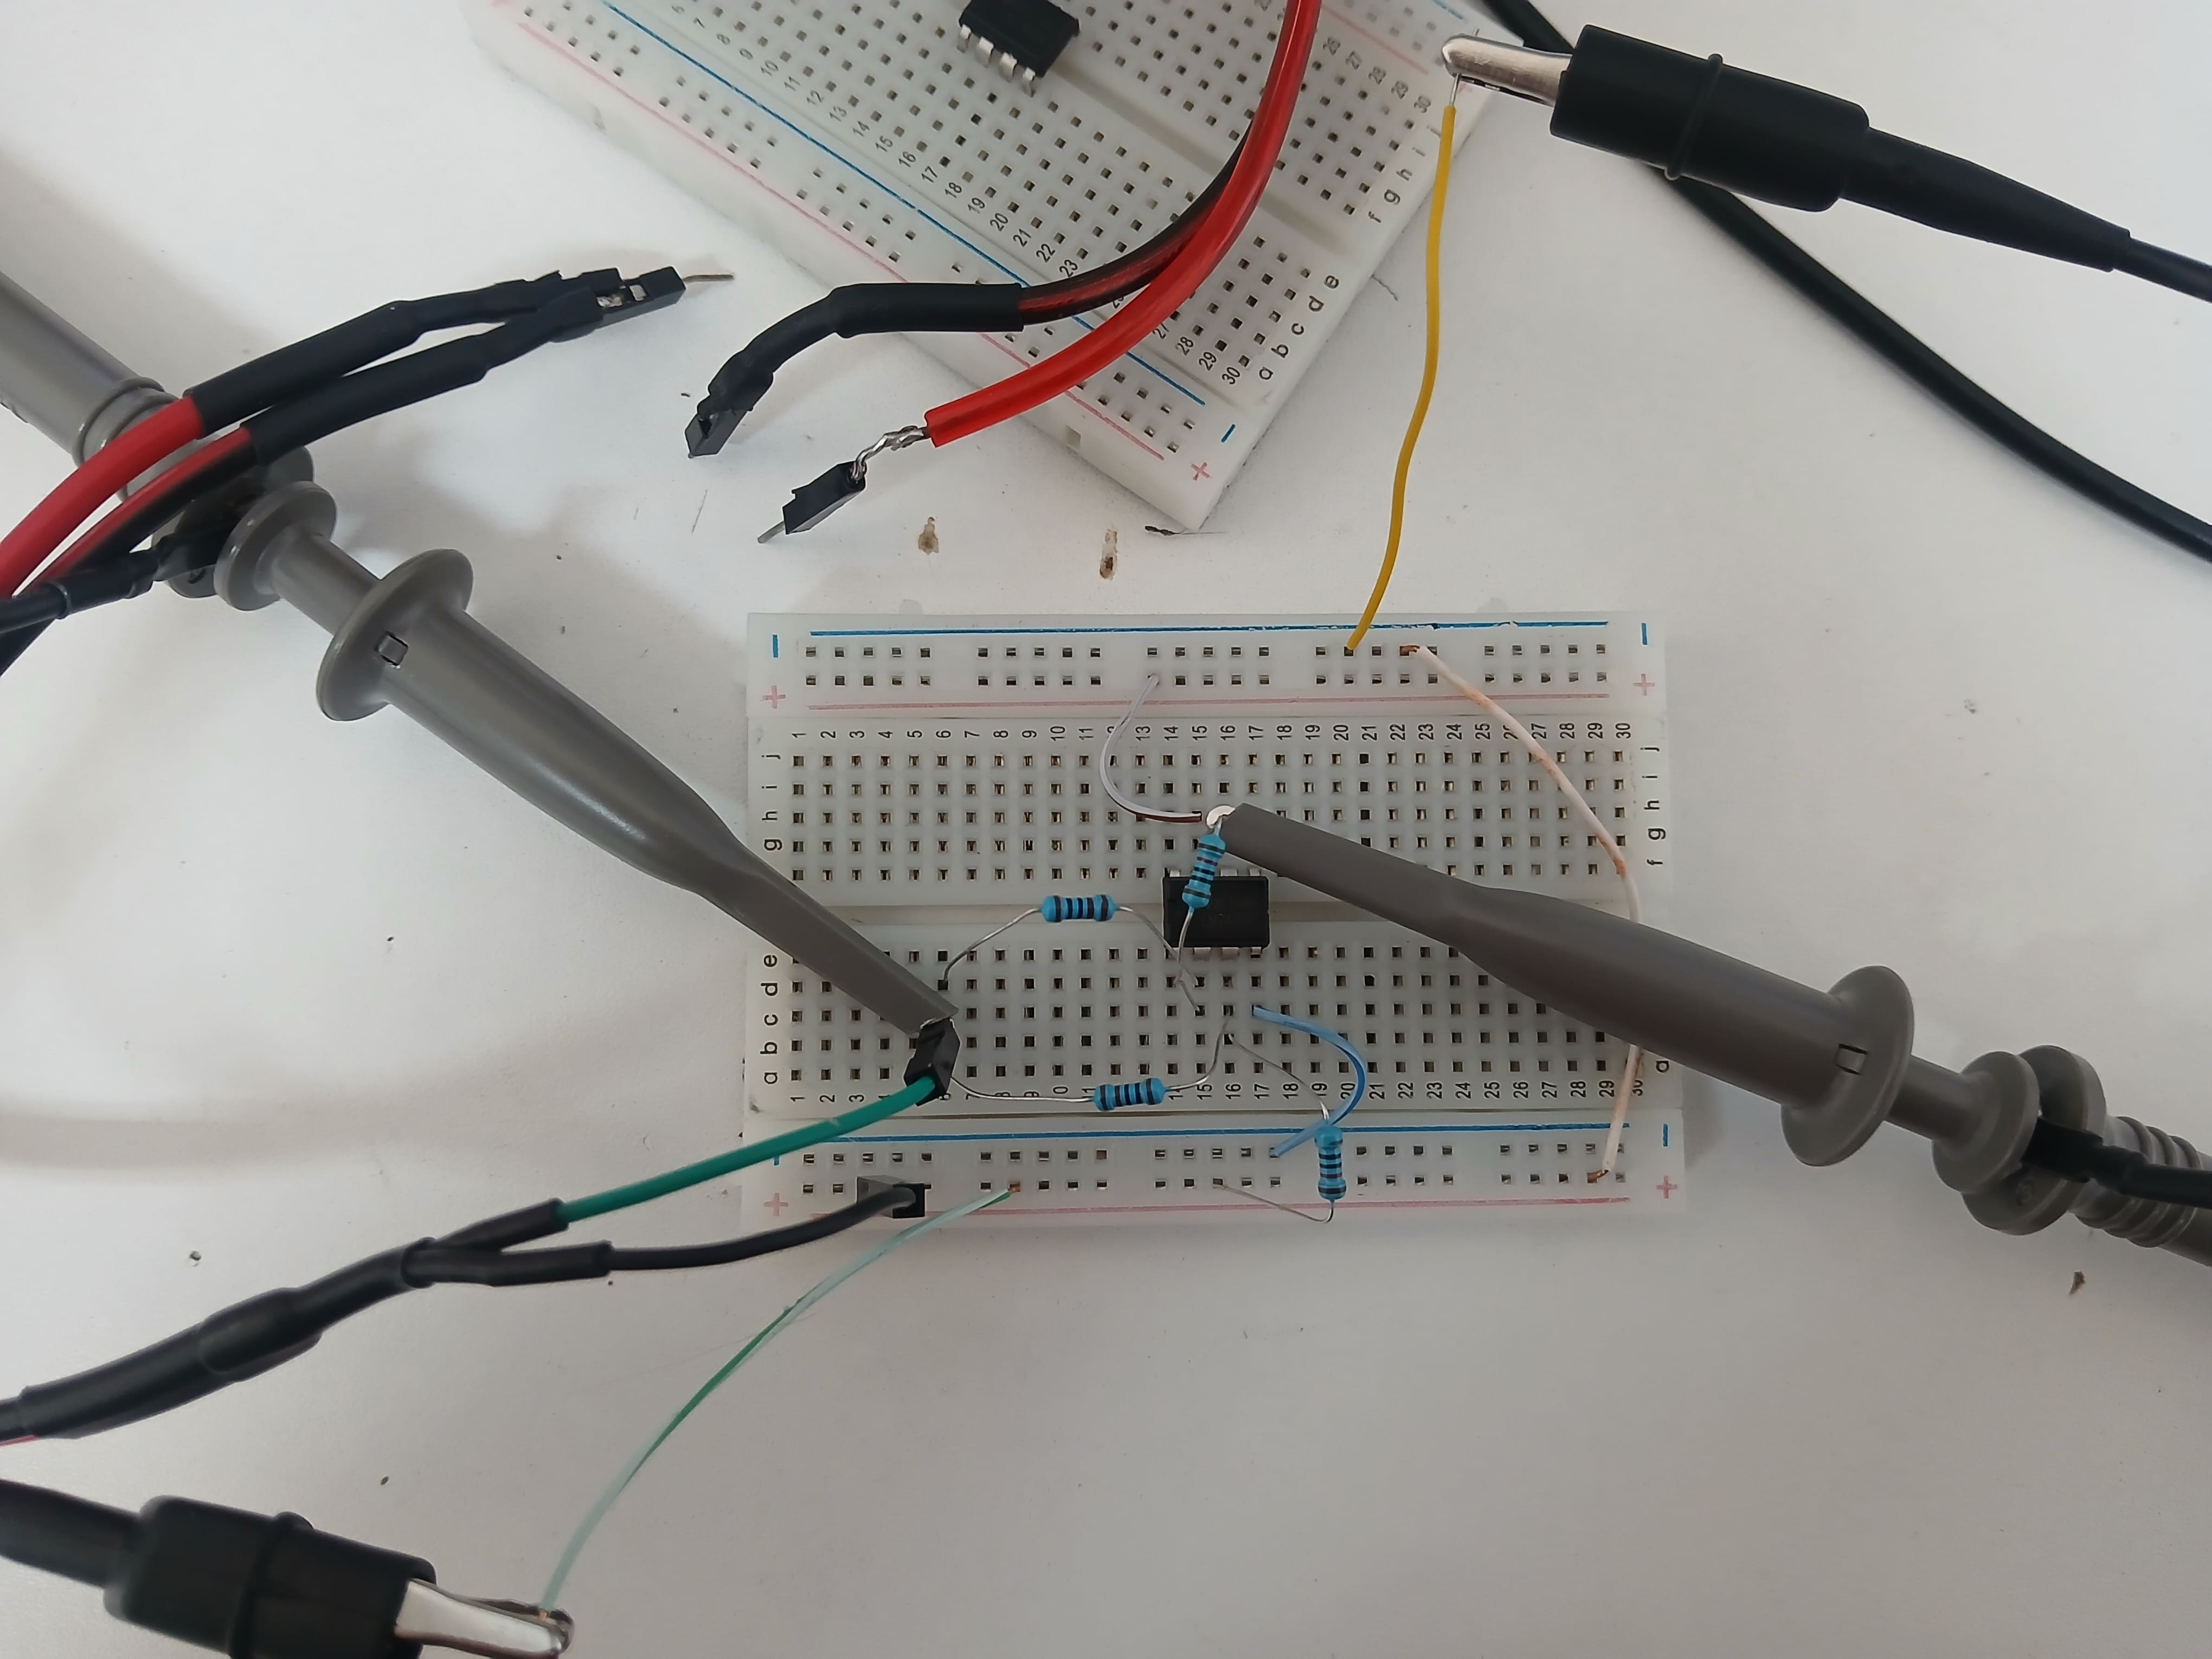
\includegraphics[width=0.5\linewidth]{media/imp-circuito-mod-comun}
	\caption{Implementación amplificador diferencial - Modo común}
	\label{fig:imp-circuito-mod-comun}
\end{figure}

Para las mediciones en el modo común se tuvo que realizar algunas modificaciones en el osciloscopio esto debido a que en este configuración el amplificador diferencial atenúa la señal común y/o ruido, viéndose esto reflejado en la escala para la entrada 2 (color celeste) del osciloscopio la cual se configuro a $100mV$ por rejilla para poder apreciar la señal sinusoidal que de otra forma (mayor escala) aparece como una señal continua (a simple vista).

Finalmente en la tabla \ref{eq:ganancia-comun} se muestran las mediciones realizadas para cada frecuencia y la atenuación definida en la misma se realiza en función a los cursores, la diferencia o variación entre estos y la amplitud en la señal de entrada.

\begin{table}[]
	\centering
	\begin{tabular}{|c|r|r|r|r|r|r|r|}
		\hline
		\textbf{F {[}Hz{]}} & \multicolumn{1}{c|}{\textbf{0,5}} & \multicolumn{1}{c|}{\textbf{5}} & \multicolumn{1}{c|}{\textbf{50}} & \multicolumn{1}{c|}{\textbf{500}} & \multicolumn{1}{c|}{\textbf{5000}} & \multicolumn{1}{c|}{\textbf{50000}} & \multicolumn{1}{c|}{\textbf{500000}} \\ \hline
		\textbf{Vc {[}V{]}} & 0,016                             & 0,016                           & 0,016                            & 0,016                             & 0,016                              & 0,032                               & 0,048                                \\ \hline
		\textbf{Ac}         & 0,032                             & 0,032                           & 0,032                            & 0,032                             & 0,032                              & 0,064                               & 0,096                                \\ \hline
	\end{tabular}
	\caption{Voltaje de salida y ganancia en modo común}
	\label{tab:ganancia-comun}
\end{table}

\section{Relación de rechazo en modo común (CMRR)}

Como se define en \cite{horenstein2000circuitos} el CMRR es la relación entre la ganancia en modo diferencial $A_d$ y  modo común $A_c$, permitiendo conocer gracias a esta característica que tan selectivo es un amplificador operacional con la señal entrada respecto a las señales de ruido, por lo tanto este valor es de vital importancia y su especificación y valor del mismo se toman como referencia para la elección de un dispositivo, matemáticamente esto se define en \ref{eq:} adimensional y en \ref{eq:} en dB.

\begin{equation}
	CMRR = \frac{A_{dm}}{A_{cm}}
	\label{eq:cmrr-adimensional}
\end{equation}

\begin{equation}
	CMRR = 20log(\frac{A_{dm}}{A_{cm}})
	\label{eq:cmrr-db}
\end{equation}

Por lo tanto ambas ganancias son de vital importancia para la obtención del CMRR y su obtención y/o calculo se realizara en base a las tablas \ref{tab:ganancia-diferencial} y \ref{tab:ganancia-comun}, compilando todo los resultados y calculo del CMRR en la tabla \ref{tab:cmrr} para las diferentes frecuencias.

\begin{table}[]
	\centering
	\begin{tabular}{|c|c|c|c|c|c|c|c|}
		\hline
		\textbf{F {[}Hz{]}}                          & \textbf{0,5} & \textbf{5} & \textbf{50} & \textbf{500} & \textbf{5000} & \textbf{50000} & \textbf{500000} \\ \hline
		\textbf{Vd {[}V{]}}                          & 4,64         & 4,72       & 4,64        & 4,72         & 4,72          & 3,44           & 0,64            \\ \hline
		\textbf{Ad {[}V{]}}                          & 9,28         & 9,44       & 9,28        & 9,44         & 9,44          & 6,88           & 1,28            \\ \hline
		\textbf{Vc {[}V{]}}                          & 0,016        & 0,016      & 0,016       & 0,016        & 0,016         & 0,032          & 0,048           \\ \hline
		\textbf{Ac {[}V{]}}                          & 0,032        & 0,032      & 0,032       & 0,032        & 0,032         & 0,064          & 0,096           \\ \hline
		\textbf{CMRR}                                & 145          & 147,5      & 145         & 147,5        & 147,5         & 53,75          & 6,67            \\ \hline
		\multicolumn{1}{|l|}{\textbf{CMRR {[}dB{]}}} & 43,23        & 43,38      & 43,23       & 43,38        & 43,38         & 34,61          & 16,48           \\ \hline
	\end{tabular}
	\caption{Ganancias diferencial, común y CMRR}
	\label{tab:cmrr}
\end{table}

\subsection{CMRR medido y especificado en la hoja de datos}

De la hoja de datos para el LM741 el valor promedio para el CMRR es de $70 dB$ como valor mínimo, siendo el valor máximo calculado en la experiencia de 43.38 dB apreciándose una considerable diferencial por lo cual el valor obtenido no estaría dentro del rango definido en el datasheet, sin embargo en el cálculo del CMRR tambièn se debe tener en cuenta las condiciones de fabrica con las cuales se realizar las pruebas y los parámetros eléctricos en la experiencia, existiendo cierta diferencia de forma puntual en el voltaje de alimentación de 12V en la hoja de datos a los 9V utilizados para la polarización, otro punto a considerar durante la experiencia son las tensiones de offset observadas en la salida la cual pudieron alterar en cierta medida las magnitudes registradas para cada caso.

Del error se puede decir que este ronda un porcentaje considerable del estimado como se demuestra a continuación:

\begin{align}
	error  = $\frac{70 - 43.38}{70}*100$ \\
	error  = 38,243
\end{align}


\section*{Resultados finales}












%%% ESTILO APA %%%%%
%--------------------

\printbibliography
%\bibliographystyle{apalike}
%\bibliography{bib.bib}
%\printbibliography

\printglossary[type=\acronymtype, title={Lista de Abreviaturas}, toctitle={Lista de Abreviaturas}]
%\printglossary[type=\acronymtype, title=T\'erminos y Abreviaturas]




\end{document}
